\chapter{Estrategia de resolución}

Este capítulo explica la estrategia de resolución seguida para resolver el problema de sincronización de semáforos en el Corredor Garzón. La metodología se basa en tres puntos: el modelado del problema, el AE multiobjetivo desarrollado y el uso de técnicas de alto desempeño para mejorar el rendimiento del algoritmo. El capítulo comienza presentando el modelo del problema, que incluye el diseño del mapa de la zona y la creación de instancias realistas que serán usadas para simular el tráfico. El capítulo describe al simulador de tráfico SUMO y el trabajo de campo realizado para recabar datos precisos de la realidad. Para finalizar se detalla la arquitectura propuesta para el diseño e implementación del AE multiobjetivo.

%Luego la sección 2 detalla la arquitectura propuesta para el diseño e implementación del algoritmo evolutivo multiobjetivo, que fue desarrollado utilizando la biblioteca Malva presentada en la sección 3. Finalmente se especifican los parámetros, características y modelo de paralelismo del Algoritmo Evolutivo implementado.


\section{Modelo del problema }

El modelado del problema comprende la simplificación de la realidad y el uso de aquellos elementos que resulten útiles para resolver el problema de sincronización de semáforos. El modelado se basa en el diseño de un mapa de la zona geográfica a estudiar y la elaboración de instancias realistas que serán usadas en el simulador de tráfico SUMO. A continuación se presenta el simulador, las herramientas necesarias utilizadas y el proceso seguido para desarrollar el modelo propuesto. 

\section{Simulaciones de tráfico}

Como se explicó en el capítulo de marco teórico, SUMO es un simulador de tráfico gratuito y de código abierto que permite modelar redes de calles, vehículos, transporte público, ciudadanos y semáforos. Este simulador sigue un modelo microscópico, ya que realiza la simulación individual explícita de cada elemento. SUMO incluye un conjunto de herramientas destinadas a facilitar la generación de tráfico y la construcción de mapas \citep{SumoTools}. 

Puesto que existe un amplio abanico de posibilidades a la hora de elegir un simulador de tráfico, se efectuó un análisis relacionado con las posibilidades y objetivos del proyecto. A continuación se presentan las razones que sustentan la elección de SUMO como el simulador de tráfico utilizado en el marco del proyecto:

\begin{itemize}
	\item Portabilidad: SUMO puede ser ejecutado tanto en Windows como en Linux. Esta característica es requerida, dado que Windows es una de las plataformas utilizadas para implementar el proyecto y Linux (CentOs) es el sistema operativo utilizado por la infraestructura computacional de alto desempeño (Cluster FING) donde se plantea desarrollar el análisis experimental.
	
	\item Disponibilidad de modos de ejecución: SUMO puede ejecutarse sin interfaz gráfica, utilizando solamente la línea de comando, lo que aumenta sensiblemente la velocidad de ejecución. Esta funcionalidad es fundamental a la hora de diseñar el AE, ya que la interacción con el simulador de tráfico debe ser eficiente. Por otro lado SUMO, presenta la opción de ejecutarse con interfaz gráfica, lo que es indispensable a la hora de visualizar la simulación. Esta opción es útil sobre todo en el inicio del desarrollo, cuando se realizan ajustes y pruebas sobre el modelo y el algoritmo.
	
	\item Software gratuito y abierto: SUMO se presenta como un proyecto de código abierto por lo que permite implementar características especificas, y no tiene costos asociados, que no podrían ser cubiertos por un proyecto estudiantil. 
	
	\item Documentación y mantenimiento: El simulador incluye una detallada documentación que hace más fácil su utilización. SUMO cuenta con una comunidad muy activa que responde dudas en los foros, lo cual es útil a la hora de buscar soporte en caso de problemas o errores. SUMO también cuenta con un desarrollo activo que permite su mejora por medio de actualizaciones frecuentes.
	
	\item Configuración simple: SUMO presenta un sencillo sistema de configuración, basada en archivos XML para la ejecución de las simulaciones. La modificación de estos archivos permiten alterar la configuración de los semáforos, las propiedades y rutas de los vehículos, entre otras opciones. Complementariamente cuenta con herramientas para importar mapas de servicios como OSM \citep{OSM}.
	
	\item Información de salida: SUMO ofrece la opción de generar una amplia variedad de datos, producida por la simulación ejecutada. Entre estos datos se encuentran la velocidad de los vehículos y el largo del recorrido, datos que son requeridos por la solución propuesta.
	
	\item Eficiencia: SUMO soporta redes de tránsito muy grandes y está diseñado para ejecutar simulaciones a gran velocidad, siendo una característica deseable por la complejidad del problema a solucionar. Un ejemplo de escenario de grandes es el \emph{``TAPAS Cologne''}, disponible públicamente en www.sumo.dlr.de/wiki , donde se describe el tráfico de la ciudad de Colonia (Alemania)  para un día entero, simulando cerca de 1.2 millones de recorridos de vehículos.
	
\end{itemize}


SUMO presenta un funcionamiento sencillo basado en tomar como entradas archivos de configuración que representan la red vial, los vehículos, el tráfico y los semáforos. Además, genera archivos de salida con información útil como el tiempo de simulación, la cantidad de vehículos, velocidad de los vehículos, duración del viaje, emisiones de gases contaminantes, etc. Una instancia de ejecución del simulador SUMO se muestra en la Figura \ref{fig:sim1}, donde se aprecia la red vial, los autos, ómnibus y paradas de ómnibus.

Dada la complejidad del problema a enfrentar en el marco del proyecto, se propone utilizar otras herramientas para realizar ciertas tareas de manera más eficiente y con menos errores. \emph{NetConvert} viene integrado con SUMO y es utilizado para generar la red vial a partir del mapa obtenido de Open Street Map, transformándolo al formato que SUMO reconoce. Otra herramienta integrada con SUMO es \emph{DUaRouter} que permite generar recorridos de vehículos basado en dinámicas definidas por el usuario. \emph{Traffic Modeler}, creado por \citet{TrafficModeler}, es útil para la generación de tráfico de manera visual que puede ser exportado al formato reconocido por SUMO. 
	


\begin{figure}[ht]
	\centering
	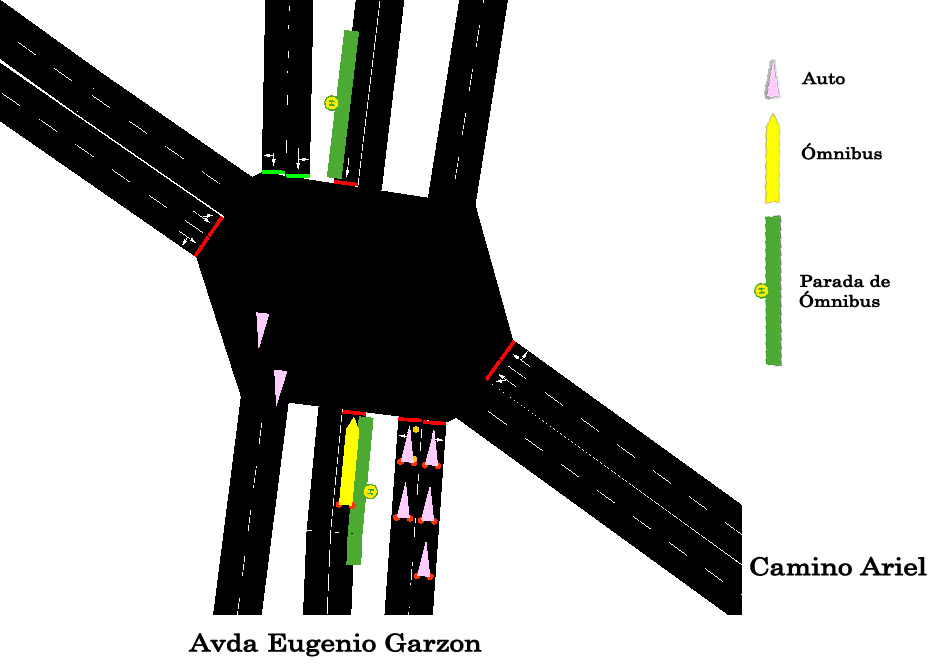
\includegraphics[width=0.9\linewidth]{Figures/sim1}
	\caption[Simulación de trafico en el simulador SUMO.]{Simulación de tráfico en el simulador SUMO en el cruce entre Bulevar Batlle y Ordoñez y el Corredor Garzón.}
	\label{fig:sim1}
\end{figure}



%\subsection{Proceso de modelado}

%El objetivo del proceso de modelado es desarrollar instancias realistas del problema. Se comienza con el diseño del mapa que representa la zona del Corredor Garzón. Luego se describe el trabajo de campo realizado para obtener datos precisos de la realidad. Finalmente utilizando estos datos, se describe el desarrollo de las instancias realistas que serán utilizadas en el simulador de tráfico.

\section{Diseño del mapa de la zona de estudio}

El primer paso del modelado consiste en diseñar un mapa de la zona del Corredor Garzón que sea compatible con el simulador. El servicio de Open Street Map \citep{OSM} cuenta con mapas libres y actualizados por una comunidad muy activa. Este servicio se utiliza para importar la zona de interés y luego editarlo con el programa JOSM (Java OpenStreetMap Editor) para poder adecuarlo a las necesidades del problema.  Se utilizaron otros servicios (Google Maps y Bing Maps) y un estudio de la zona para validar la exactitud del mapa importado desde OSM. El estudio consistió en recorrer el Corredor Garzón, analizando en cada intersección: las reglas de cruce utilizadas y las direcciones de circulación de las calles. Como resultado de la verificación in situ fueron detectadas algunas inconsistencias entre la realidad y el mapa importado. Todas las inconsistencias detectadas fueron corregidas en la versión del mapa a utilizar en el proyecto. 

El alcance geográfico de la zona de estudio comprende al Corredor Garzón en toda su extensión y dos caminos paralelos a cada lado del mismo. Como se ve en el mapa de la Figura \ref{fig:mapa_osm_sumo}, no existen calles paralelas reales, por lo que el proceso para diseñar el mapa consistió en: \textit{i)} seleccionar las calles que construyen dos caminos paralelos a cada lado del Corredor Garzón; \textit{ii)} seleccionar las calles internas entre las paralelas, verificando que cada camino paralelo incluya calles doble mano o dos calles de una sola mano, \textit{iii)} finalmente se borran las demás calles que no están incluidas en la zona modelada.

Dado los cambios realizados en el mapa, como la eliminación de calles que no formaban parte de la zona modelada, no se pudo contribuir con la comunidad OSM subiendo el mapa con las modificaciones que corregían algunas inconsistencias encontradas.



\begin{figure}[H]
	\centering
	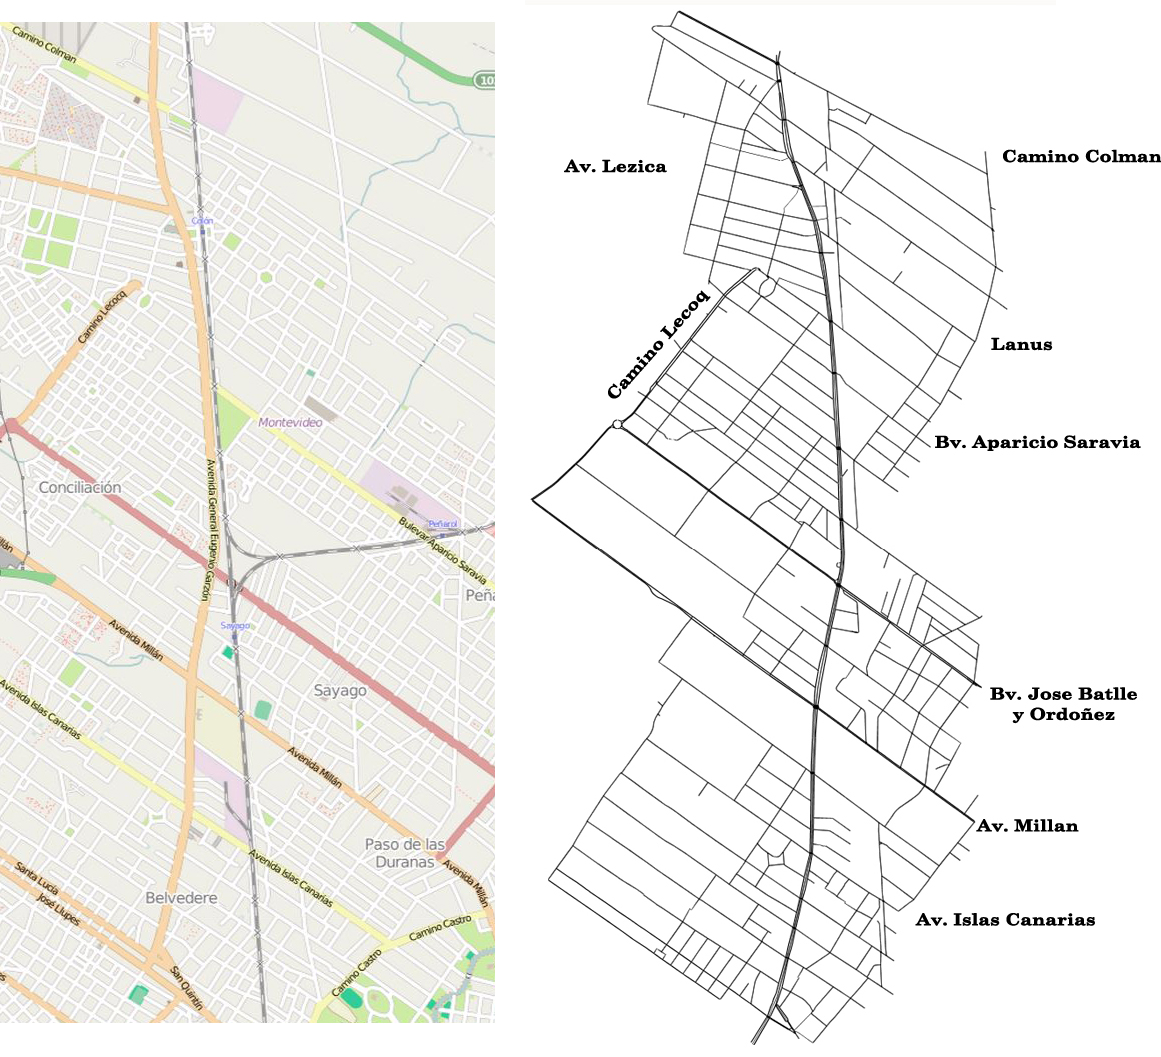
\includegraphics[width=0.9\linewidth]{Figures/mapa_osm_sumo}
	\caption[Mapa del corredor Garzón]{Mapa del corredor Garzón. A la izquierda el mapa extraído de OSM, a la derecha el mapa procesado listo para ser usado en SUMO. El corredor Garzón está en el centro de cada imagen.}
	\label{fig:mapa_osm_sumo}
\end{figure}

La herramienta \emph{Netconvert} fue utilizada para transformar el mapa obtenido desde OSM al formato XML que reconoce el simulador SUMO. Esta herramienta no reconoce algunos datos incluidos en el formato OSM, por ejemplo los números de las casas, las vías de tren, las vías de peatones, los caminos, las plazas, las paradas de ómnibus y los separadores que tiene el corredor de las vías para autos, entre otros. Se destaca como punto importante que NetConvert no reconoce correctamente a los corredores, ya que confunde y superpone el corredor central con las vías para los autos, seguramente por no reconocer los separadores físicos que presenta el corredor. Para solucionar este problema se utilizó el programa JOSM para eliminar los datos no reconocidos por NetConvert y editar el mapa, separando aproximadamente un metro las calles del corredor central.

La modificación realizada permitió que \emph{NetConvert} interpretara correctamente el funcionamiento del corredor, para que los vehículos no se trasladaran entre la vía de los autos y la del corredor de ómnibus. Sin embargo, el cambio implementado generó un problema, ya que cada cruce de la realidad pasó a ser representado por tres cruces distintos (uno por cada calle del corredor). Para solucionar el problema anterior y otros errores relacionados a las reglas de circulación en las intersecciones, se realizaron ajustes manuales, modificando los archivos XML relacionados. Entre otros cambios, se especificaron manualmente las reglas de movilidad correctas en algunos cruces, por ejemplo cuando estaba prohibido girar a la izquierda.

Al finalizar el proceso de diseño se obtuvo un mapa fiel a la realidad, delimitado en la zona del Corredor Garzón, que es compatible con el simulador de tráfico SUMO. Al importar el mapa desde OSM y transformarlo con \emph{NetConvert} se genera una configuración de semáforos por defecto que no es correcta t será corregida mas adelante utilizando los datos relevados in situ; proceso que se explica a continuación.


\section{Recolección de datos en trabajo de campo}

Existen datos públicos disponibles en el sitio web de la Intendencia de Montevideo (www.montevideo.gub.uy) sobre la cantidad de ómnibus y sus frecuencias, pero no se tienen datos sobre la densidad del tráfico vehicular en la zona del Corredor Garzón. Por este motivo se realizó un revelamiento in-situ en cinco cruces representativos de la zona estudiada; cada cruce representa una intersección de vías entre el Corredor Garzón y una calle en particular. Los cruces seleccionados fueron: Camino Ariel, Batlle y Ordoñez, Plaza Vidella, Camino Colman y Aparicio Saravia. Estos cruces presentan diferentes características que son útiles para modelar variantes en la cantidad de vehículos circulantes. 

En el relevamiento de tráfico se siguieron las recomendaciones de los textos consultados relacionados con el conteo vehicular \citep{ConteoTrafico}. El día seleccionado para efectuar el conteo fué el miércoles, con clima soleado y en el horario de 15:00 a 17:00 horas, para no obtener sesgos que se producen los fines de semana, en horas pico, o en días de lluvia. Se realizaron filmaciones de entre 15 y 30 minutos en los cruces y luego se analizaron los vídeos para efectuar el conteo manual con la posibilidad de enlentecer el vídeo para mayor facilidad del conteo. Luego se completó una planilla electrónica con el formato presentado en la Figura \ref{fig:conteo_hoja}, donde se reportan la cantidad de vehículos que recorren el Corredor Garzón, los que circulan por la calle que cruza y los que doblan en cada intersección. 

\begin{figure}[ht]
	\centering
	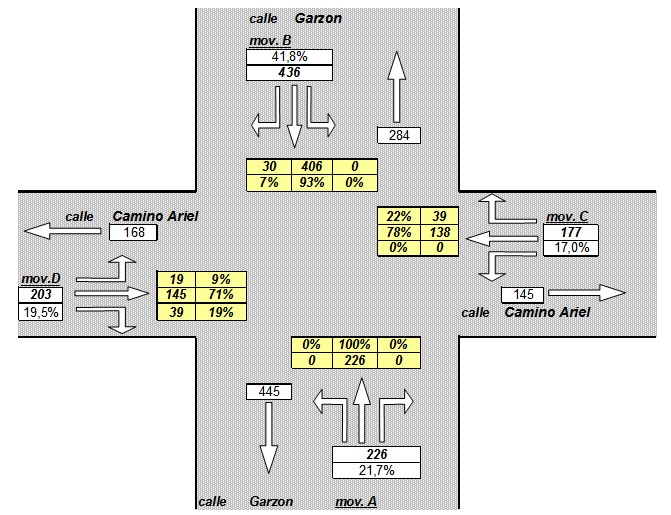
\includegraphics[width=0.9\linewidth]{Figures/conteo_hoja}
	\caption[Ejemplo de planilla electrónica para el conteo manual de tráfico.]{Ejemplo de planilla electrónica para el conteo manual de tráfico en la intersección entre el corredor Garzón y Camino Ariel}
	\label{fig:conteo_hoja}
\end{figure}



\begin{table}[ht]
	\renewcommand{\arraystretch}{1.2}
	\caption[Resumen del revelamiento del tráfico en la zona del corredor Garzón.]{Resumen del revelamiento del tráfico en la zona del corredor Garzón. Se muestra la cantidad de vehículos y la orientación hacia donde circulan.}
	\label{table:resumen_trafico}
	\centering
	\begin{tabular}{lcccc}
		\hline
		Intersección&
		Sur-Garzón& 
		Norte-Garzón & 
		Oeste &
		Este 
		\\ 
		\hline
		Camino Colman  & 410 & 390 & 140 & 230\\		
		Plaza Vidiella  & 400 & 444 & 292 & 0\\		
		Aparicio Saravia  & 390 & 450 & 40 & 90\\		
		Batlle y Ordoñez  & 510 & 390 & 470 & 300 \\	
		Camino Ariel  & 436 & 226 & 177 & 203 \\													
		\hline
		
		
		\hline
	\end{tabular}
\end{table}

La tabla \ref{table:resumen_trafico} muestra la cantidad de vehículos contados en los distintos cruces; hay que tener en cuenta que solamente se contabilizan los autos, no se tienen en cuenta otro tipo de vehículos. Esta decisión se basa en un relevamiento preliminar de la zona que constató que la cantidad de otros vehículos (camiones, motos, bicicletas, etc) no era significante en el total del tráfico (menos de 10 \%), por lo que no se justificaba su adición al conteo y a la posterior simulación del tráfico.

Complementariamente al procedimiento de conteo manual, se realizaron recorridas de punta a punta del corredor a una velocidad constante en auto, para tomar datos de demora a ser utilizados a la hora de desarrollar las simulaciones de tráfico. Con este análisis se obtiene tanto la duración total del recorrido como el tiempo que un vehículo permanece detenido en los cruces semaforizados. 

Para la configuración de los semáforos, se realizó un recorrido (en bicicleta) por toda la extensión del Corredor Garzón. Se cronometró la duración de las luces de los semáforos en cada esquina recorriendo el camino de ida, y para validar los tiempos también se relevaron las duraciones de las luces en el camino de vuelta. Estos tiempos fueron verificados por los vídeos obtenidos anteriormente en el conteo del tráfico.


\section{Desarrollo de instancias realistas del problema}

Una vez completado el diseño del mapa compatible con el simulador de la zona del Corredor Garzón, y obtenidos los datos relevados de la realidad, se procedió al desarrollo de instancias realistas que representen la situación actual en relación con el tráfico. Estas instancias representan los escenarios que serán simulados en el simulador de tráfico. Para configurar la simulación del tráfico se utilizan como entrada tres archivos de configuración en formato XML que son reconocidos por el simulador SUMO. El primero es el archivo de \emph{configuración de los semáforos} donde se detalla la duración de las luces, el comienzo de fase y la ubicación de los mismos en el mapa base. El segundo archivo representa la \emph{ruta de los vehículos} que contiene el recorrido de cada vehículo. Finalmente el tercer archivo con el \emph{recorrido de los ómnibus} indica el recorrido de los mismos, su frecuencia, la ubicación de las paradas, en cuáles se detienen y el tiempo que demoran en la parada. Estas tres etapas serán explicadas en detalle a continuación.

\subsection{Configuración de semáforos}

El diseño del mapa genera una configuración de semáforos por defecto que no es correcta, por tanto, se corrige utilizando los datos relevados previamente sobre las duraciones de las luces y las fases de los semáforos de cada intersección del Corredor Garzón. La modificación se realiza sobre un archivo XML que representa la configuración de semáforos de todo el Corredor Garzón, que será utilizado como archivo de entrada a la hora de realizar las simulaciones de tráfico.

\subsection{Generación de tráfico vehicular}

Existen varios modelos disponibles para representar la circulación de los vehículos. El modelo \emph{aleatorio} genera recorridos para los vehículos al azar. En el modelo \emph{basado en áreas} se especifican las zonas donde el tráfico se origina y donde finaliza. Un modelo más complejo es el \emph{basado en actividad}, donde se definen la cantidad de casas, el número de vehículos y la población de una zona determinada. Luego, el modelo genera la densidad de tráfico basado en los tipos de actividades que se realizan comúnmente, como ir al trabajo, hacer las compras, ir a la escuela, etc. Finalmente, un modelo muy utilizado, sobre todo en escenarios de tamaño reducido, es el \emph{definido por el usuario}, que permite determinar la ruta de cada vehículo con mayor detalle.

Se utilizó el programa \emph{Traffic Modeler} \citep{TrafficModeler} que se caracteriza por generar modelos de tráfico complejos de manera visual como se ve en la Figura \ref{fig:areaflow1}. Se optó por un modelo de movilidad entre áreas, lo que permite una buena granularidad al especificar la densidad de tráfico. 

Para generar múltiples instancias con distintas configuraciones de tráfico, en el \emph{Traffic Modeler} se especifican la cantidad de autos y las áreas entre las cuales se movilizan, utilizando el mapa base diseñado previamente, luego el programa genera los recorridos que son exportados en un archivo. Este archivo es procesado con la herramienta \emph{duaRouter} (incluido en SUMO) para generar otro archivo que contiene las rutas especificas de cada recorrido de los autos. El archivo resultante será incluido al ejecutar las simulaciones de tráfico.


%El programa genera el recorrido del viaje para cada vehículo, que se mantiene constantes en las distintas ejecuciones del algoritmo evolutivo. La variación se produce en las velocidades desarrolladas por cada uno, ya que dependiendo de la configuración de los semáforos logrará mayores o menores velocidades.



\begin{figure}[ht]
	\centering
	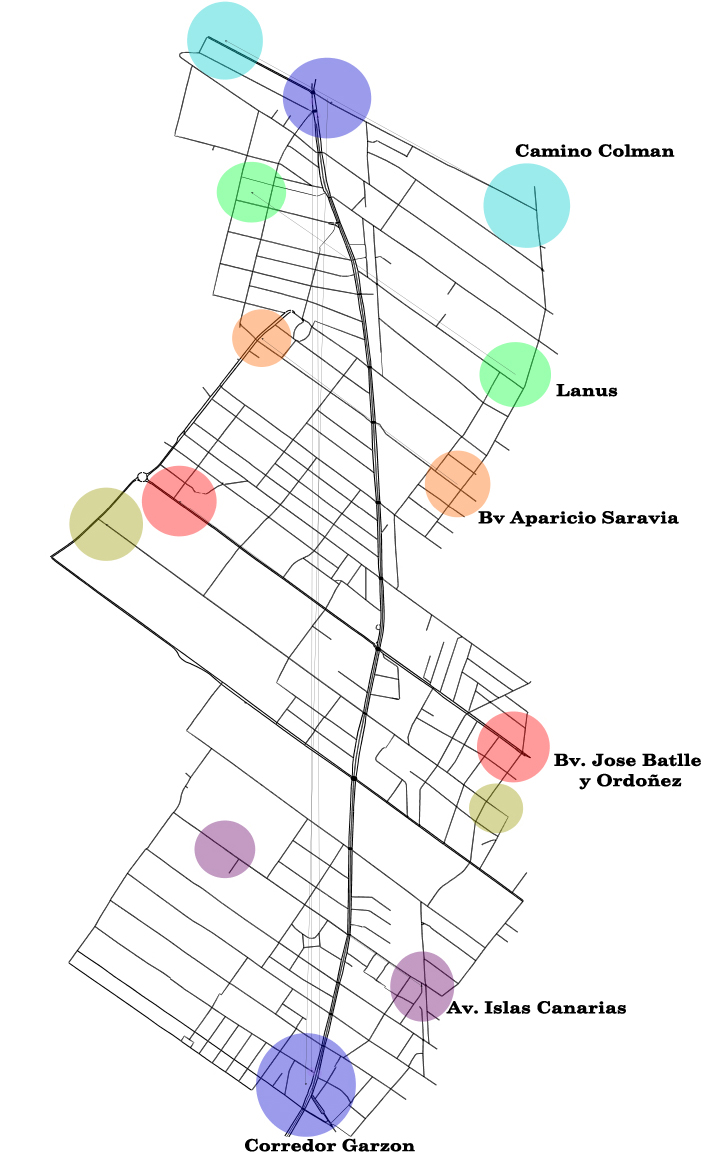
\includegraphics[width=0.5\linewidth]{Figures/areaflow1}
	\caption[Mapa diseñado en el TrafficModeler para la generación de tráfico.]{Mapa diseñado en el TrafficModeler para la generación de trafico. Los círculos del mismo color especifican el tráfico entre esas áreas. }
	\label{fig:areaflow1}
\end{figure}

\subsection{Generación de recorridos de ómnibus}

Se plantea el uso de dos tipos de vehículos: autos y ómnibus. Cada tipo de vehículo posee diferentes características asociadas, como el tamaño, la aceleración y la velocidad máxima. No se especifican otros tipos de vehículos como motos o camiones, ya que su proporción respecto al total de tráfico en la zona del Corredor Garzón no lo justificaba. Las frecuencias y los distintos recorridos de los ómnibus, fueron obtenidos de datos públicos de la Intendencia Municipal de Montevideo (IMM). Las frecuencias incluyen las líneas urbanas: 'G', '409' ,'2', 'D5'  y  '148'. Las líneas de ómnibus suburbanas no utilizan el carril exclusivo central, sino las calles adyacentes provocando un comportamiento diferente al de las líneas urbanas. Por este motivo las velocidades de las líneas suburbanas no serán tomadas en cuenta en la evaluación de la función de \emph{fitness} del algoritmo evolutivo, para no generar distorsiones en los resultados.

La ubicación y líneas de cada parada se obtuvo del Servicio de Información Geográfica de Montevideo (http://sig.montevideo.gub.uy). Existen 14 paradas de líneas urbanas por el Corredor Garzón para el recorrido de ida y la misma cantidad para el recorrido de vuelta. Se tuvo en cuenta para los recorridos de los ómnibus las detenciones en las paradas y el tiempo que demora detenido, por ejemplo existen paradas donde se demora más tiempo por la cantidad de pasajeros que ascienden y descienden. Las duraciones de las detenciones en cada parada fueron calculadas utilizando los vídeos realizados en el trabajo de campo para el relevamiento del tráfico, donde se cronometraron los tiempos que demoraban las detenciones en las paradas. De este estudio se calcularon los tiempo de detención en las paradas, que se encuentran en el rango de 15 a 35 segundos.

Se realizó un estudio basado en datos de GPS proporcionados por la IMM. Estos datos cuentan con la posición exacta, la velocidad instantánea y la referencia del ómnibus, para un conjunto de líneas seleccionadas tomadas en un período de una semana. 
Para este procesamiento se utilizó QGIS (www.qgis.org), un sistema de información geográfico capaz de visualizar, editar y realizar operaciones sobre elementos geográficos. Adicionalmente fue necesario el desarrollo de \emph{scripts} para obtener las estadísticas necesarias, ya que la cantidad de información estudiada era muy grande (1.5Gb). El uso de QGIS permitió seleccionar, filtrar y relacionar los datos de posición y velocidad con las líneas que circulan por el Corredor Garzón. Luego de procesar los datos se constató una velocidad media de 14.5 km/h en el Corredor Garzón, lo que permitió ajustar mejor el modelo. 


\subsection{Resumen}

Una vez obtenidos los archivos con la configuración de los semáforos, el recorrido de los vehículos y el recorrido de los ómnibus, se cuenta con todos los elementos necesarios para la creación de instancias realistas del problema, que serán utilizadas en el simulador para modelar la realidad.  En el análisis experimental presentado en el capítulo 5 se describen los escenarios que hacen uso de estas instancias, modificando algunas variables como la densidad del tráfico para ajustarlo a las necesidades de la experimentación.



\section{Arquitectura de la solución}


El problema de optimización que se pretende resolver es el de maximizar las velocidades promedio de ómnibus y vehículos en la zona del Corredor Garzón. Como se busca optimizar dos objetivos al mismo tiempo se plantea el uso de un enfoque de optimización multiobjetivo. Para implementar este enfoque, se utiliza una combinación lineal de los objetivos (velocidad de ómnibus y de vehículos), ya que es un método sencillo y adecuado para problemas de optimización que involucran menos de tres objetivos y el frente de Pareto del problema es convexo \citep{coello2002evolutionary}.



\begin{figure}[ht]
	\centering
	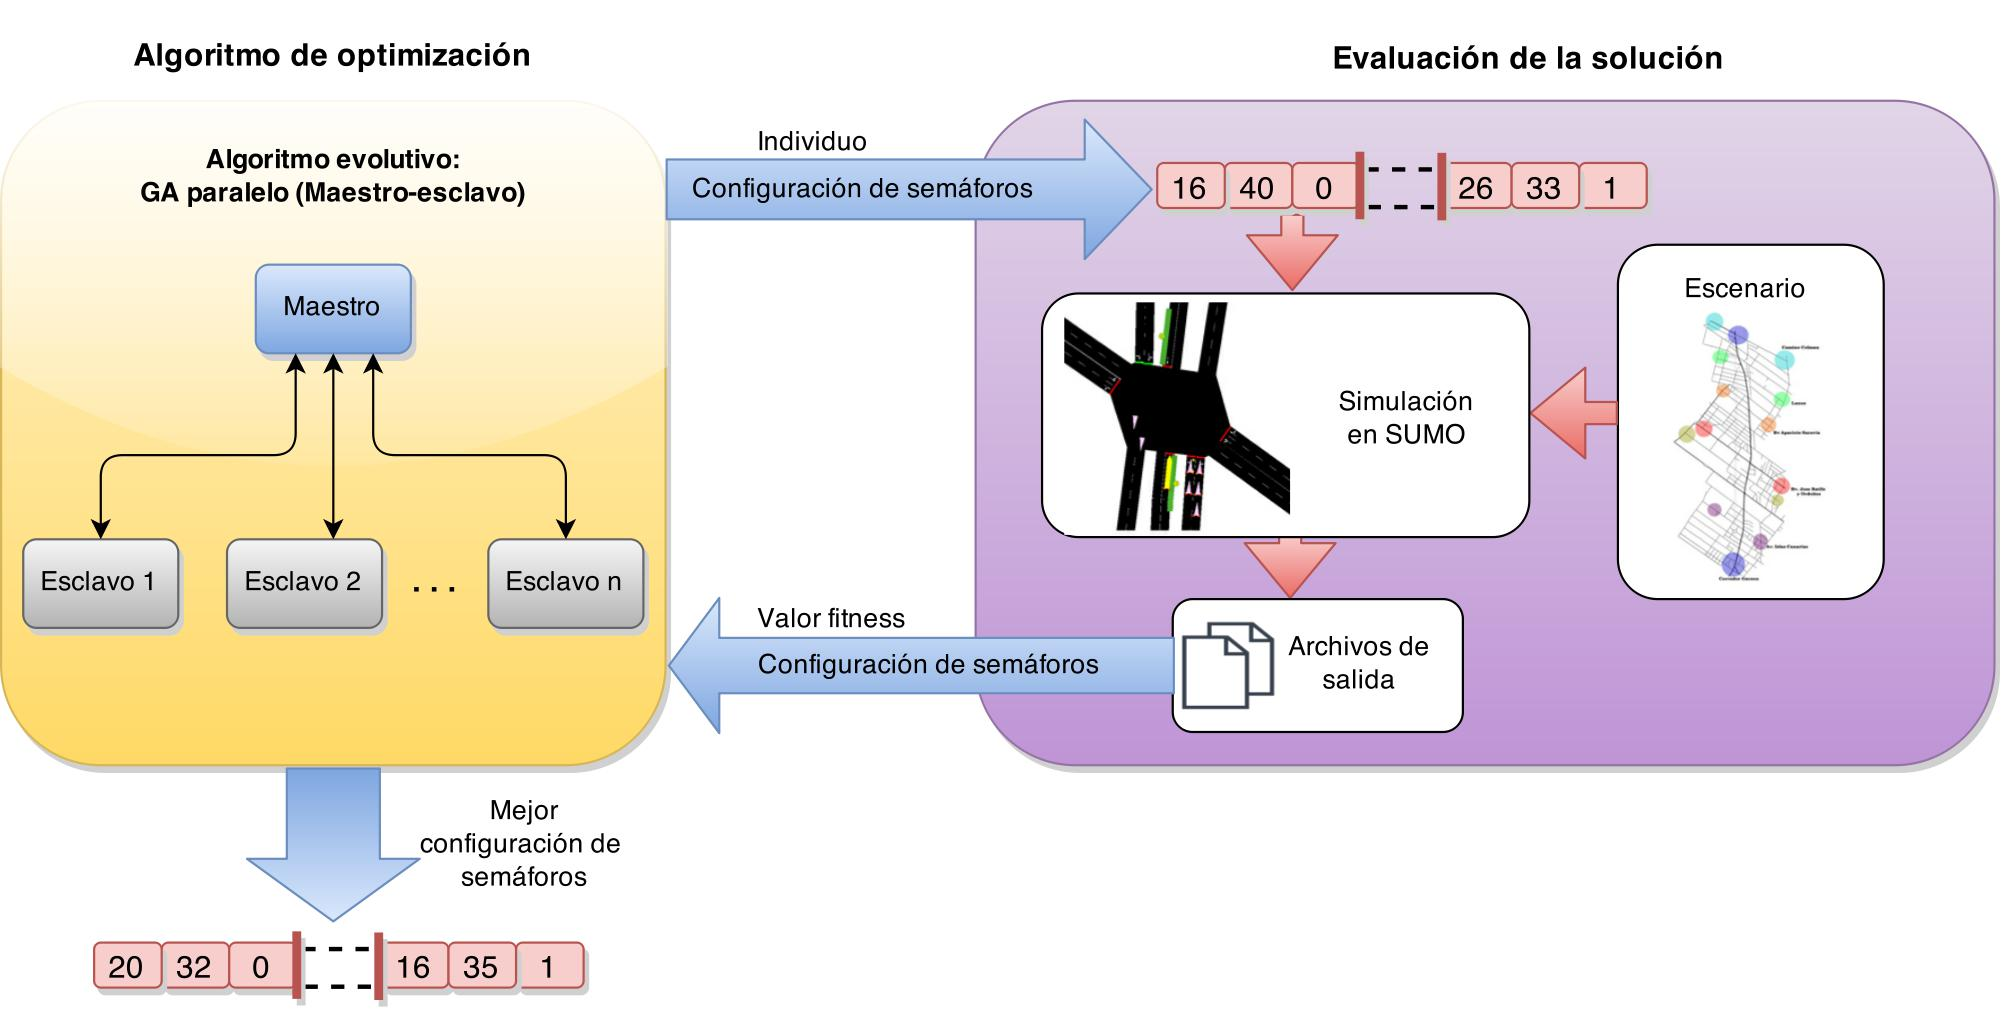
\includegraphics[width=0.99\linewidth]{Figures/arquitectura1}
	\caption{Arquitectura de la solución propuesta.}
	\label{fig:arquitectura1}
\end{figure}

El esquema de la Figura \ref{fig:arquitectura1}  muestra la arquitectura propuesta para la resolución del problema. La arquitectura se puede dividir en dos grandes bloques que interactuan entre sí, por un lado el algoritmo de optimización y por otro la evaluación de la solución. El AE implementa paralelismo con un enfoque maestro-esclavo. El primer paso consiste en generar la población inicial del AE, estos individuos representan una configuración de semáforos para todo el Corredor Garzón, que incluye la duración de las fases y el \emph{offset}. Luego, por cada individuo se genera un archivo compatible con el simulador, que representa la configuración de semáforos. Este archivo se utiliza como entrada para ejecutar el simulador al momento de evaluar la función de \emph{fitness}, como se aprecia en la flecha azul hacia la derecha de la Figura \ref{fig:arquitectura1}. Estas evaluaciones se realizan en paralelo, por lo que pueden existir tantas evaluaciones ejecutando al mismo tiempo como individuos en la población. Al finalizar la ejecución del simulador SUMO se generan archivos de salida que son enviados hacia el AE, específicamente hacia cada uno de los esclavos, como indica la flecha azul que apunta hacia la izquierda en la Figura \ref{fig:arquitectura1}. Los datos de salida incluyen información necesaria para calcular el \emph{fitness} de cada individuo como la velocidad media de ómnibus y otros vehículos. El proceso maestro consolida los datos enviados por los esclavos, y aplica los operadores evolutivos, para continuar con la siguiente iteración. El AE se detiene al alcanzar un número de generaciones determinado, en ese momento se crea un archivo con la mejor configuración de semáforos encontrada, que corresponde a la mejor solución del problema de optimización planteado. 






